% Options for packages loaded elsewhere
\PassOptionsToPackage{unicode}{hyperref}
\PassOptionsToPackage{hyphens}{url}
\PassOptionsToPackage{dvipsnames,svgnames,x11names}{xcolor}
%
\documentclass[
  a4paper,
]{article}

\usepackage{amsmath,amssymb}
\usepackage{iftex}
\ifPDFTeX
  \usepackage[T1]{fontenc}
  \usepackage[utf8]{inputenc}
  \usepackage{textcomp} % provide euro and other symbols
\else % if luatex or xetex
  \usepackage{unicode-math}
  \defaultfontfeatures{Scale=MatchLowercase}
  \defaultfontfeatures[\rmfamily]{Ligatures=TeX,Scale=1}
\fi
\usepackage{lmodern}
\ifPDFTeX\else  
    % xetex/luatex font selection
\fi
% Use upquote if available, for straight quotes in verbatim environments
\IfFileExists{upquote.sty}{\usepackage{upquote}}{}
\IfFileExists{microtype.sty}{% use microtype if available
  \usepackage[]{microtype}
  \UseMicrotypeSet[protrusion]{basicmath} % disable protrusion for tt fonts
}{}
\makeatletter
\@ifundefined{KOMAClassName}{% if non-KOMA class
  \IfFileExists{parskip.sty}{%
    \usepackage{parskip}
  }{% else
    \setlength{\parindent}{0pt}
    \setlength{\parskip}{6pt plus 2pt minus 1pt}}
}{% if KOMA class
  \KOMAoptions{parskip=half}}
\makeatother
\usepackage{xcolor}
\usepackage[top=2.54cm,right=2.54cm,bottom=2.54cm,left=2.54cm]{geometry}
\setlength{\emergencystretch}{3em} % prevent overfull lines
\setcounter{secnumdepth}{-\maxdimen} % remove section numbering
% Make \paragraph and \subparagraph free-standing
\ifx\paragraph\undefined\else
  \let\oldparagraph\paragraph
  \renewcommand{\paragraph}[1]{\oldparagraph{#1}\mbox{}}
\fi
\ifx\subparagraph\undefined\else
  \let\oldsubparagraph\subparagraph
  \renewcommand{\subparagraph}[1]{\oldsubparagraph{#1}\mbox{}}
\fi


\providecommand{\tightlist}{%
  \setlength{\itemsep}{0pt}\setlength{\parskip}{0pt}}\usepackage{longtable,booktabs,array}
\usepackage{calc} % for calculating minipage widths
% Correct order of tables after \paragraph or \subparagraph
\usepackage{etoolbox}
\makeatletter
\patchcmd\longtable{\par}{\if@noskipsec\mbox{}\fi\par}{}{}
\makeatother
% Allow footnotes in longtable head/foot
\IfFileExists{footnotehyper.sty}{\usepackage{footnotehyper}}{\usepackage{footnote}}
\makesavenoteenv{longtable}
\usepackage{graphicx}
\makeatletter
\def\maxwidth{\ifdim\Gin@nat@width>\linewidth\linewidth\else\Gin@nat@width\fi}
\def\maxheight{\ifdim\Gin@nat@height>\textheight\textheight\else\Gin@nat@height\fi}
\makeatother
% Scale images if necessary, so that they will not overflow the page
% margins by default, and it is still possible to overwrite the defaults
% using explicit options in \includegraphics[width, height, ...]{}
\setkeys{Gin}{width=\maxwidth,height=\maxheight,keepaspectratio}
% Set default figure placement to htbp
\makeatletter
\def\fps@figure{htbp}
\makeatother

% Preámbulo
\usepackage{comment} % Permite comentar secciones del código
\usepackage{marvosym} % Agrega símbolos adicionales
\usepackage{graphicx} % Permite insertar imágenes
\usepackage{mathptmx} % Fuente de texto matemática
\usepackage{amssymb} % Símbolos adicionales de matemáticas
\usepackage{lipsum} % Crea texto aleatorio
\usepackage{amsthm} % Teoremas y entornos de demostración
\usepackage{float} % Control de posiciones de figuras y tablas
\usepackage{rotating} % Rotación de elementos
\usepackage{multirow} % Celdas combinadas en tablas
\usepackage{tabularx} % Tablas con ancho de columna ajustable
\usepackage{mdframed} % Marcos alrededor de elementos flotantes

% Series de tiempo
\usepackage{booktabs}


% Configuración adicional

\makeatletter
\makeatother
\makeatletter
\makeatother
\makeatletter
\@ifpackageloaded{caption}{}{\usepackage{caption}}
\AtBeginDocument{%
\ifdefined\contentsname
  \renewcommand*\contentsname{Tabla de contenidos}
\else
  \newcommand\contentsname{Tabla de contenidos}
\fi
\ifdefined\listfigurename
  \renewcommand*\listfigurename{Listado de Figuras}
\else
  \newcommand\listfigurename{Listado de Figuras}
\fi
\ifdefined\listtablename
  \renewcommand*\listtablename{Listado de Tablas}
\else
  \newcommand\listtablename{Listado de Tablas}
\fi
\ifdefined\figurename
  \renewcommand*\figurename{Figura}
\else
  \newcommand\figurename{Figura}
\fi
\ifdefined\tablename
  \renewcommand*\tablename{Tabla}
\else
  \newcommand\tablename{Tabla}
\fi
}
\@ifpackageloaded{float}{}{\usepackage{float}}
\floatstyle{ruled}
\@ifundefined{c@chapter}{\newfloat{codelisting}{h}{lop}}{\newfloat{codelisting}{h}{lop}[chapter]}
\floatname{codelisting}{Listado}
\newcommand*\listoflistings{\listof{codelisting}{Listado de Listados}}
\makeatother
\makeatletter
\@ifpackageloaded{caption}{}{\usepackage{caption}}
\@ifpackageloaded{subcaption}{}{\usepackage{subcaption}}
\makeatother
\makeatletter
\@ifpackageloaded{tcolorbox}{}{\usepackage[skins,breakable]{tcolorbox}}
\makeatother
\makeatletter
\@ifundefined{shadecolor}{\definecolor{shadecolor}{rgb}{.97, .97, .97}}
\makeatother
\makeatletter
\makeatother
\makeatletter
\makeatother
\ifLuaTeX
\usepackage[bidi=basic]{babel}
\else
\usepackage[bidi=default]{babel}
\fi
\babelprovide[main,import]{spanish}
% get rid of language-specific shorthands (see #6817):
\let\LanguageShortHands\languageshorthands
\def\languageshorthands#1{}
\ifLuaTeX
  \usepackage{selnolig}  % disable illegal ligatures
\fi
\usepackage[]{biblatex}
\addbibresource{../../../../references.bib}
\IfFileExists{bookmark.sty}{\usepackage{bookmark}}{\usepackage{hyperref}}
\IfFileExists{xurl.sty}{\usepackage{xurl}}{} % add URL line breaks if available
\urlstyle{same} % disable monospaced font for URLs
\hypersetup{
  pdftitle={Explorando la Elasticidad. Entendiendo las Dinámicas del Mercado},
  pdfauthor={Edison Achalma},
  pdflang={es},
  colorlinks=true,
  linkcolor={blue},
  filecolor={Maroon},
  citecolor={Blue},
  urlcolor={Blue},
  pdfcreator={LaTeX via pandoc}}

\title{Explorando la Elasticidad. Entendiendo las Dinámicas del Mercado}
\usepackage{etoolbox}
\makeatletter
\providecommand{\subtitle}[1]{% add subtitle to \maketitle
  \apptocmd{\@title}{\par {\large #1 \par}}{}{}
}
\makeatother
\subtitle{Elasticidad}
\author{Edison Achalma}
\date{2023-06-23}

\begin{document}
\maketitle
\ifdefined\Shaded\renewenvironment{Shaded}{\begin{tcolorbox}[interior hidden, enhanced, boxrule=0pt, sharp corners, borderline west={3pt}{0pt}{shadecolor}, breakable, frame hidden]}{\end{tcolorbox}}\fi

\hypertarget{introducciuxf3n-a-la-elasticidad}{%
\section{Introducción a la
Elasticidad}\label{introducciuxf3n-a-la-elasticidad}}

\hypertarget{quuxe9-es-la-elasticidad}{%
\subsection{¿Qué es la elasticidad?}\label{quuxe9-es-la-elasticidad}}

La elasticidad es un concepto fundamental en economía que nos ayuda a
comprender cómo responden la demanda y la oferta ante cambios en los
precios y otros factores. En pocas palabras, nos permite medir la
sensibilidad de la cantidad demandada o ofrecida ante variaciones en
determinadas variables.

Imagina que el precio de un producto aumenta. ¿Qué sucederá con la
cantidad que las personas están dispuestas a comprar? La elasticidad nos
proporciona una medida para responder a esta pregunta. Si la demanda es
elástica, significa que los consumidores son sensibles a los cambios en
el precio y reducirán su consumo en gran medida. Por otro lado, si la
demanda es inelástica, significa que los consumidores son menos
sensibles y continuarán comprando a pesar del aumento de precio.

La elasticidad es una herramienta poderosa que nos ayuda a entender cómo
funciona el mercado y cómo los cambios en variables clave pueden afectar
las decisiones de los consumidores y las empresas. En los siguientes
fragmentos, exploraremos diferentes tipos de elasticidad y su aplicación
práctica en el mundo empresarial. ¡Vamos a sumergirnos en el fascinante
mundo de la elasticidad económica!

\hypertarget{importancia-de-la-elasticidad-en-la-economuxeda}{%
\subsection{Importancia de la elasticidad en la
economía}\label{importancia-de-la-elasticidad-en-la-economuxeda}}

La elasticidad es un concepto clave en la economía porque nos permite
comprender cómo cambian las decisiones y el comportamiento de los
consumidores y las empresas frente a los cambios en los precios y otros
factores económicos.

Imagina que eres propietario de un negocio y estás considerando aumentar
el precio de tus productos. Antes de tomar esa decisión, es fundamental
comprender cómo reaccionarán los consumidores. Aquí es donde entra en
juego la elasticidad. Si la demanda es elástica, un aumento en el precio
podría resultar en una disminución significativa de las ventas, lo que
podría afectar negativamente tus ingresos. Por otro lado, si la demanda
es inelástica, un aumento en el precio podría tener un impacto menor en
las ventas, lo que te brinda una mayor flexibilidad para ajustar tus
precios.

Además, la elasticidad también nos ayuda a comprender los efectos de los
impuestos, las políticas gubernamentales y otros factores en la
economía. Por ejemplo, si se impone un impuesto a un producto, la
elasticidad nos permite predecir cómo afectará la demanda y cuánto
ingreso generará el impuesto.

\hypertarget{tipos-de-elasticidad}{%
\subsection{Tipos de elasticidad}\label{tipos-de-elasticidad}}

Existen varios tipos de elasticidad que nos ayudan a comprender
diferentes aspectos del comportamiento de la demanda y la oferta. Cada
tipo de elasticidad se centra en una variable específica y nos
proporciona información única sobre cómo responden los agentes
económicos a los cambios en esa variable.

\begin{enumerate}
\def\labelenumi{\arabic{enumi}.}
\item
  \textbf{Elasticidad precio de la demanda:} Esta medida nos indica cómo
  responde la cantidad demandada de un bien o servicio a cambios en su
  precio. Si la demanda es elástica, significa que los consumidores son
  sensibles a las variaciones de precio y una pequeña alteración en el
  precio puede tener un gran impacto en la cantidad demandada. Por otro
  lado, si la demanda es inelástica, significa que los consumidores son
  menos sensibles al cambio de precio.
\item
  \textbf{Elasticidad ingreso de la demanda:} Esta medida nos indica
  cómo responde la cantidad demandada de un bien o servicio a cambios en
  el ingreso de los consumidores. Si la demanda es elástica con respecto
  al ingreso, significa que la cantidad demandada aumentará en
  proporción mayor al incremento del ingreso. Por el contrario, si la
  demanda es inelástica, significa que la cantidad demandada no
  aumentará significativamente ante un incremento en el ingreso.
\item
  \textbf{Elasticidad cruzada de la demanda:} Esta medida nos indica
  cómo responde la cantidad demandada de un bien o servicio ante cambios
  en el precio de otro bien o servicio relacionado. Si la elasticidad
  cruzada de la demanda es positiva, significa que los bienes son
  sustitutos y un aumento en el precio de uno de ellos conducirá a un
  aumento en la demanda del otro. Si la elasticidad cruzada es negativa,
  significa que los bienes son complementarios y un aumento en el precio
  de uno de ellos reducirá la demanda del otro.
\item
  \textbf{Elasticidad precio de la oferta:} Esta medida nos indica cómo
  responde la cantidad ofrecida de un bien o servicio a cambios en su
  precio. Si la oferta es elástica, significa que los productores pueden
  aumentar la cantidad ofrecida en respuesta a un aumento en el precio.
  Si la oferta es inelástica, significa que los productores no pueden
  aumentar significativamente la cantidad ofrecida incluso ante un
  aumento en el precio.
\end{enumerate}

En los próximos fragmentos, exploraremos cada tipo de elasticidad en más
detalle y veremos cómo se aplican en situaciones reales.

\hypertarget{elasticidad-precio-de-la-demanda}{%
\section{Elasticidad Precio de la
Demanda}\label{elasticidad-precio-de-la-demanda}}

\hypertarget{concepto-y-fuxf3rmula-de-la-elasticidad-precio-de-la-demanda}{%
\subsection{Concepto y fórmula de la elasticidad precio de la
demanda}\label{concepto-y-fuxf3rmula-de-la-elasticidad-precio-de-la-demanda}}

La elasticidad precio de la demanda es una medida importante en economía
que nos permite entender cómo cambia la cantidad demandada de un bien o
servicio ante variaciones en su precio. Esta medida nos ayuda a
comprender la sensibilidad de los consumidores frente a los cambios de
precio.

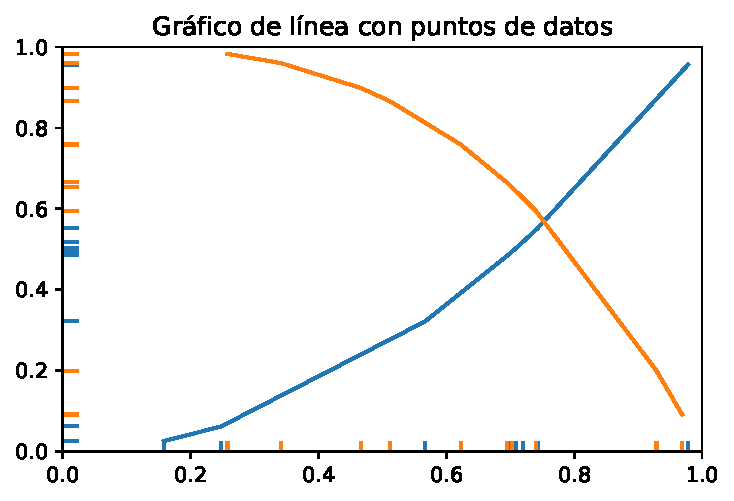
\includegraphics{index_files/figure-pdf/cell-2-output-1.pdf}

Las diferentes fórmulas de la elasticidad precio de la demanda son las
siguientes:

\begin{equation}\protect\hypertarget{eq-1}{}{
Elasticidad precio de la demanda =\frac{\% cambio en la cantidad demandada}{\% cambio en el precio}
}\label{eq-1}\end{equation}

la Ecuación~\ref{eq-1} nos muestra cómo medir la elasticidad.
Simplemente dividimos el porcentaje de cambio en la cantidad demandada
entre el porcentaje de cambio en el precio.

\[
\eta _{XP_y} = \frac{\frac {X_f^d - X_i^d}{X_i}}{\frac {P_f^d - P_i^d}{P_i^d}}
\]

\[
= \frac{\frac{\Delta X^d}{X_i^d}}{\frac{\Delta P_x^d}{P_i^d}}
\]

\begin{equation}\protect\hypertarget{eq-2}{}{
= \frac{\Delta X^d P_i^d}{\Delta P_x^d X_i^d}
}\label{eq-2}\end{equation}

La Ecuación~\ref{eq-2} nos permite calcular la elasticidad precio de la
demanda utilizando los cambios absolutos en la cantidad demandada y el
precio inicial. Dividimos la diferencia entre la cantidad final y la
cantidad inicial por la cantidad inicial, y hacemos lo mismo con la
diferencia entre el precio final y el precio inicial, dividiéndola por
el precio inicial.

\begin{equation}\protect\hypertarget{eq-3}{}{
\eta _{PX^d} = \frac{\partial X^d P_x}{\partial P_x X^d}
}\label{eq-3}\end{equation}

La Ecuación~\ref{eq-3} se basa en el cálculo de derivadas parciales. Nos
permite medir la elasticidad precio de la demanda considerando los
cambios infinitesimales en la cantidad demandada y el precio.

\begin{equation}\protect\hypertarget{eq-4}{}{
\eta _{PX^d} = \frac{\partial \ln(\mathrm X)}{\partial  \ln(\mathrm P_x)}
}\label{eq-4}\end{equation}

La Ecuación~\ref{eq-4} utiliza logaritmos naturales para calcular la
elasticidad. Tomamos las derivadas parciales de los logaritmos de la
cantidad demandada y el precio para obtener la elasticidad.
\begin{equation}\protect\hypertarget{eq-5}{}{
\eta _{PX^d} = \frac{\Delta \% X^d}{\Delta \% P_x}
}\label{eq-5}\end{equation}

La Ecuación~\ref{eq-5} nos muestra cómo medir la elasticidad utilizando
los cambios porcentuales en la cantidad demandada y el precio.

\begin{equation}\protect\hypertarget{eq-6}{}{
\eta_{PX^d} = m_{ip} \frac{P_i^d}{X^d}
}\label{eq-6}\end{equation}

La Ecuación~\ref{eq-6} introduce el concepto de pendiente de la curva de
demanda. Multiplicamos la pendiente de la curva por el precio inicial
dividido por la cantidad demandada para obtener la elasticidad.

Estas fórmulas nos brindan diferentes enfoques para calcular la
elasticidad precio de la demanda, y cada una tiene su utilidad en
diferentes contextos. Es importante comprender cómo aplicarlas y qué
información nos brindan para tomar decisiones estratégicas en el ámbito
económico.

\hypertarget{interpretaciuxf3n-de-la-elasticidad-precio-de-la-demanda}{%
\subsection{Interpretación de la elasticidad precio de la
demanda}\label{interpretaciuxf3n-de-la-elasticidad-precio-de-la-demanda}}

Una vez que comprendemos qué es la elasticidad precio de la demanda y
cómo se calcula, es importante poder interpretar los resultados
obtenidos. La elasticidad nos brinda información valiosa sobre la
sensibilidad de los consumidores ante cambios en el precio de un
producto. Veamos cómo interpretar los distintos valores de la
elasticidad:

\begin{itemize}
\item
  Elasticidad mayor a 1: Si la elasticidad es mayor a 1, se dice que la
  demanda es elástica. Esto significa que los consumidores son muy
  sensibles al cambio de precio. Un pequeño aumento en el precio puede
  resultar en una disminución significativa en la cantidad demandada, y
  viceversa. En este caso, es crucial para las empresas considerar
  cuidadosamente los ajustes de precios, ya que podrían tener un impacto
  considerable en la demanda.
\item
  Elasticidad igual a 1: Si la elasticidad es igual a 1, se dice que la
  demanda es unitaria. Esto implica que los cambios en el precio tienen
  un impacto proporcional en la cantidad demandada. Por ejemplo, si el
  precio aumenta en un 10\%, la cantidad demandada disminuirá en un
  10\%. En este caso, las empresas deben tener en cuenta que cualquier
  cambio en el precio tendrá un efecto equivalente en la demanda.
\item
  Elasticidad menor a 1: Si la elasticidad es menor a 1, se dice que la
  demanda es inelástica. Esto indica que los consumidores son menos
  sensibles a los cambios en el precio. Incluso si el precio aumenta, la
  cantidad demandada disminuirá en una proporción menor. Aquí, las
  empresas pueden tener más flexibilidad para ajustar los precios sin
  experimentar una caída drástica en la demanda.
\end{itemize}

Es importante destacar que la elasticidad precio de la demanda puede
variar según el producto, el mercado y el momento. Por lo tanto, es
esencial realizar análisis específicos para comprender cómo los cambios
en el precio afectarán la demanda en situaciones particulares.

Ejemplo

\[
X^d = \frac{P_y P_z I^{0.2} N}{2 P_x}
\]

Aplicando la fórmula Ecuación~\ref{eq-2}

\[ 
\eta _{PX^d} = \frac{\partial \mathrm{X}}{\partial \mathrm{P_x}} \frac{\mathrm{P_x}}{\mathrm{X^d}} 
\]

\[
= - \frac{P_y P_z I^{0.2} N}{2 (P_x)^2} \frac{\mathrm{P_x}}{\mathrm{X^d} }
\]

reemplazamos \(x^d\) con su valor \[
= - \frac{P_y P_z I^{0.2} N}{2 (P_x)^2} \frac{\mathrm{P_x}}{\frac{P_y P_z I^{0.2} N}{2 P_x} }
\]

ordenando y resolviendo

\[
= - \frac{2 P_y P_z (P_x)^2 I^{0.2} N}{2 P_y P_z (P_x)^2 I^{0.2} N} = -1
\]

interpretación

Si el \(P_x\) aumenta en 1\% entonces \(X^d\) disminuye en 1\%.

\hypertarget{factores-que-influyen-en-la-elasticidad-precio-de-la-demanda}{%
\subsection{Factores que influyen en la elasticidad precio de la
demanda}\label{factores-que-influyen-en-la-elasticidad-precio-de-la-demanda}}

\hypertarget{elasticidad-precio-de-la-oferta}{%
\section{Elasticidad Precio de la
Oferta}\label{elasticidad-precio-de-la-oferta}}

\hypertarget{significado-y-cuxe1lculo-de-la-elasticidad-precio-de-la-oferta}{%
\subsection{Significado y cálculo de la elasticidad precio de la
oferta}\label{significado-y-cuxe1lculo-de-la-elasticidad-precio-de-la-oferta}}

\hypertarget{anuxe1lisis-de-la-elasticidad-precio-de-la-oferta-en-diferentes-industrias}{%
\subsection{Análisis de la elasticidad precio de la oferta en diferentes
industrias}\label{anuxe1lisis-de-la-elasticidad-precio-de-la-oferta-en-diferentes-industrias}}

\hypertarget{determinantes-de-la-elasticidad-precio-de-la-oferta}{%
\subsection{Determinantes de la elasticidad precio de la
oferta}\label{determinantes-de-la-elasticidad-precio-de-la-oferta}}

\hypertarget{elasticidad-cruzada}{%
\section{Elasticidad Cruzada}\label{elasticidad-cruzada}}

\hypertarget{definiciuxf3n-y-fuxf3rmula-de-la-elasticidad-cruzada}{%
\subsection{Definición y fórmula de la elasticidad
cruzada}\label{definiciuxf3n-y-fuxf3rmula-de-la-elasticidad-cruzada}}

\hypertarget{interpretaciuxf3n-de-la-elasticidad-cruzada}{%
\subsection{Interpretación de la elasticidad
cruzada}\label{interpretaciuxf3n-de-la-elasticidad-cruzada}}

\hypertarget{aplicaciones-pruxe1cticas-de-la-elasticidad-cruzada}{%
\subsection{Aplicaciones prácticas de la elasticidad
cruzada}\label{aplicaciones-pruxe1cticas-de-la-elasticidad-cruzada}}

\hypertarget{elasticidad-ingreso-de-la-demanda}{%
\section{Elasticidad Ingreso de la
Demanda}\label{elasticidad-ingreso-de-la-demanda}}

\hypertarget{explicaciuxf3n-y-cuxe1lculo-de-la-elasticidad-ingreso-de-la-demanda}{%
\subsection{Explicación y cálculo de la elasticidad ingreso de la
demanda}\label{explicaciuxf3n-y-cuxe1lculo-de-la-elasticidad-ingreso-de-la-demanda}}

\hypertarget{impacto-de-la-elasticidad-ingreso-en-los-patrones-de-consumo}{%
\subsection{Impacto de la elasticidad ingreso en los patrones de
consumo}\label{impacto-de-la-elasticidad-ingreso-en-los-patrones-de-consumo}}

\hypertarget{factores-que-afectan-la-elasticidad-ingreso-de-la-demanda}{%
\subsection{Factores que afectan la elasticidad ingreso de la
demanda}\label{factores-que-afectan-la-elasticidad-ingreso-de-la-demanda}}

\hypertarget{aplicaciones-de-la-elasticidad-en-la-toma-de-decisiones-empresariales}{%
\section{Aplicaciones de la Elasticidad en la Toma de Decisiones
Empresariales}\label{aplicaciones-de-la-elasticidad-en-la-toma-de-decisiones-empresariales}}

\hypertarget{uso-de-la-elasticidad-en-la-fijaciuxf3n-de-precios}{%
\subsection{Uso de la elasticidad en la fijación de
precios}\label{uso-de-la-elasticidad-en-la-fijaciuxf3n-de-precios}}

\hypertarget{estrategias-de-marketing-basadas-en-la-elasticidad}{%
\subsection{Estrategias de marketing basadas en la
elasticidad}\label{estrategias-de-marketing-basadas-en-la-elasticidad}}

\hypertarget{estudio-de-casos-ejemplos-reales-de-la-aplicaciuxf3n-de-la-elasticidad-en-empresas}{%
\subsection{Estudio de casos: Ejemplos reales de la aplicación de la
elasticidad en
empresas}\label{estudio-de-casos-ejemplos-reales-de-la-aplicaciuxf3n-de-la-elasticidad-en-empresas}}

\hypertarget{conclusiones-y-reflexiones-finales}{%
\section{Conclusiones y Reflexiones
Finales}\label{conclusiones-y-reflexiones-finales}}

\hypertarget{recapitulaciuxf3n-de-los-conceptos-clave}{%
\subsection{Recapitulación de los conceptos
clave}\label{recapitulaciuxf3n-de-los-conceptos-clave}}

\hypertarget{importancia-de-comprender-la-elasticidad-para-la-toma-de-decisiones}{%
\subsection{Importancia de comprender la elasticidad para la toma de
decisiones}\label{importancia-de-comprender-la-elasticidad-para-la-toma-de-decisiones}}

\hypertarget{reflexiones-sobre-la-aplicabilidad-y-relevancia-de-la-elasticidad-en-el-mundo-actual}{%
\subsection{Reflexiones sobre la aplicabilidad y relevancia de la
elasticidad en el mundo
actual}\label{reflexiones-sobre-la-aplicabilidad-y-relevancia-de-la-elasticidad-en-el-mundo-actual}}

\hypertarget{publicaciones-similares}{%
\section{Publicaciones Similares}\label{publicaciones-similares}}

Si te interesó este artículo, te recomendamos que explores otros blogs y
recursos relacionados que pueden ampliar tus conocimientos. Aquí te dejo
algunas sugerencias:

\begin{enumerate}
\def\labelenumi{\arabic{enumi}.}
\item
  \href{../2023-06-12-introducion-organizacion-industrial-oi-cap1/index.qmd}{Introducción
  a organización industrial}
\item
  \href{../2023-06-13-empresa-como-organizacion-oi-cap1/index.qmd}{La
  Empresa como Organización. Promoviendo Valores Cooperativos, Humanos y
  Sociales}
\item
  \href{../2023-06-13-sistemas-economicos-oi.cap1/index.qmd}{Introducción
  a los Sistemas Económicos. Cómo se distribuyen los recursos y se
  producen}
\item
  \href{../2023-06-15-mercado-relevante-oi-cap2/index.qmd}{El Mercado
  Relevante Industrial de Bienes y el Mercado Geográfico}
\item
  \href{../2023-06-16-concentracion-poder-oi-cap3/index.qmd}{Medidas de
  concentracion}
\item
  \href{../2023-06-17-estructura-mercado-oi-cap4/index.qmd}{Estructura
  de mercado}
\end{enumerate}

Esperamos que encuentres estas publicaciones igualmente interesantes y
útiles. ¡Disfruta de la lectura!


\printbibliography


\end{document}
